\section{Arquitectura Delta}

\subsection{Principios de Diseño}

Todo el almacenamiento de datos a largo plazo se realiza en un formato de tabla abierta, 
que combina archivos en formato Parquet con un registro de transacciones. 
Esto garantiza propiedades ACID y permite operaciones confiables en entornos distribuidos. \newline

Al utilizar object storage, se logra una separación clara entre los recursos de procesamiento y los de almacenamiento, 
lo que permite escalarlos de manera independiente. \newline

Además, múltiples clientes pueden acceder a los mismos datos de forma simultánea sin interferencias, 
incluso utilizando herramientas diferentes, siempre que sean compatibles con el formato subyacente.\newline

El formato Parquet, al ser columnar, permite ejecutar consultas SQL de manera eficiente 
y es compatible con la mayoría de los motores de análisis modernos. \newline

El procesamiento de datos se gestiona como un flujo continuo de eventos, 
donde el motor de procesamiento utiliza el log de transacciones como fuente de verdad para mantener el estado de los datos. 
Esto permite unificar el procesamiento batch y streaming en una misma arquitectura.
Como efecto secundario de esto, todos los datos son guardados para cada etapa del flujo de procesamiento. 
Esto significa que están disponibles para su fácil consumo en caso de que se quieran analizar; 
pero como contraparte, consumen más espacio de almacenamiento ya que se almacena potencialmente varias veces el mismo dato (aunque enriquecido). \newline

Además, el sistema se encarga automáticamente de optimizaciones como la compactación de archivos pequeños
y la gestión eficiente de metadatos, asegurando un rendimiento óptimo sin intervención manual.\newline

Por último, al estar basado en estándares abiertos, el sistema evita el vendor lock-in 
y permite integración con diversas herramientas de BI, machine learning y ETL.

\newpage
\subsection{Stack Tecnológico}
Para la capa de ingesta y transporte de datos se implementó \textbf{Apache Kafka}, 
un sistema de mensajería distribuido que proporciona alta durabilidad, replicación y garantía en el orden de los eventos. 
Kafka actúa como el punto de entrada de la arquitectura, permitiendo desacoplar la ingesta de datos del procesamiento 
y asegurando una capa de buffer que absorbe picos de tráfico mientras mantiene los datos disponibles para su consumo.
En este caso, Kafka se despliega en un cluster de tres nodos, con un factor de replicación de tres y un factor de partición de tres.
Por otro lado, se definió un tiempo de retención de mensajes acotado, en este caso de 7 días, para evitar la acumulación de datos
pero a su vez, asegurar la disponibilidad de los mismos para su procesamiento.\newline

El procesamiento de datos se realiza mediante \textbf{Apache Flink}, se despliega en un cluster con un nodo Job Manager 
y cinco nodos Task Manager; de forma de distribuir la carga de trabajo lo mejor posible.
En este caso, se define como punto de entrada un tópico de Kafka, para luego continuar procesando los datos, 
no utilizando Kafka sino aprovechando las capacidades de \textbf{Apache Paimon}. 
Este adopta un enfoque log-structured para las escrituras, 
lo que lo hace eficiente para cargas de trabajo de streaming con alta frecuencia de actualizaciones.\newline

Este permite tratar una tabla de datos como un flujo continuo de eventos, funcionando de forma efectiva como 
una cola de mensajes, pero con la ventaja de tener los datos materializados en un almacenamiento persistente y barato.\newline

Por último, este formato de almacenamiento permite ser leido por \textbf{Apache Doris}, un motor de análisis de datos
distribuido que permite realizar consultas SQL en tiempo real sobre grandes volúmenes de datos con una interfaz basada en MySQL.\newline

Para esto, tanto como para el uso de Flink, se necesita definir un catálogo de tablas.
Normalmente, esto podría hacerse utilizando Apache Hive, pero se optó por simplificar el sistema tanto como sea posible, 
y dado que no se necesitaba interactuar con un sistema existente; por lo que el catálogo se almacenó en Object Storage.\newline
\newpage
Esto último se logró mediante el uso de \textbf{MinIO}, un servidor de almacenamiento de objetos de código abierto que
permite almacenar datos de forma segura y eficiente, y que además es compatible con el protocolo S3 de Amazon Web Services.\newline

Esta combinación tecnológica permite implementar efectivamente los principios de la Arquitectura Delta, 
donde los datos fluyen desde las fuentes a través de Kafka, son procesados por Flink, 
almacenados en diferentes capas mediante Paimon sobre MinIO, y finalmente consultados a través de Doris, 
manteniendo en todo momento las propiedades ACID 
y permitiendo el procesamiento continuo así como análisis retrospectivos sobre datos históricos.

\newpage
\subsection{Vista de Componentes}


\begin{figure}[h]
    \makebox[\textwidth]{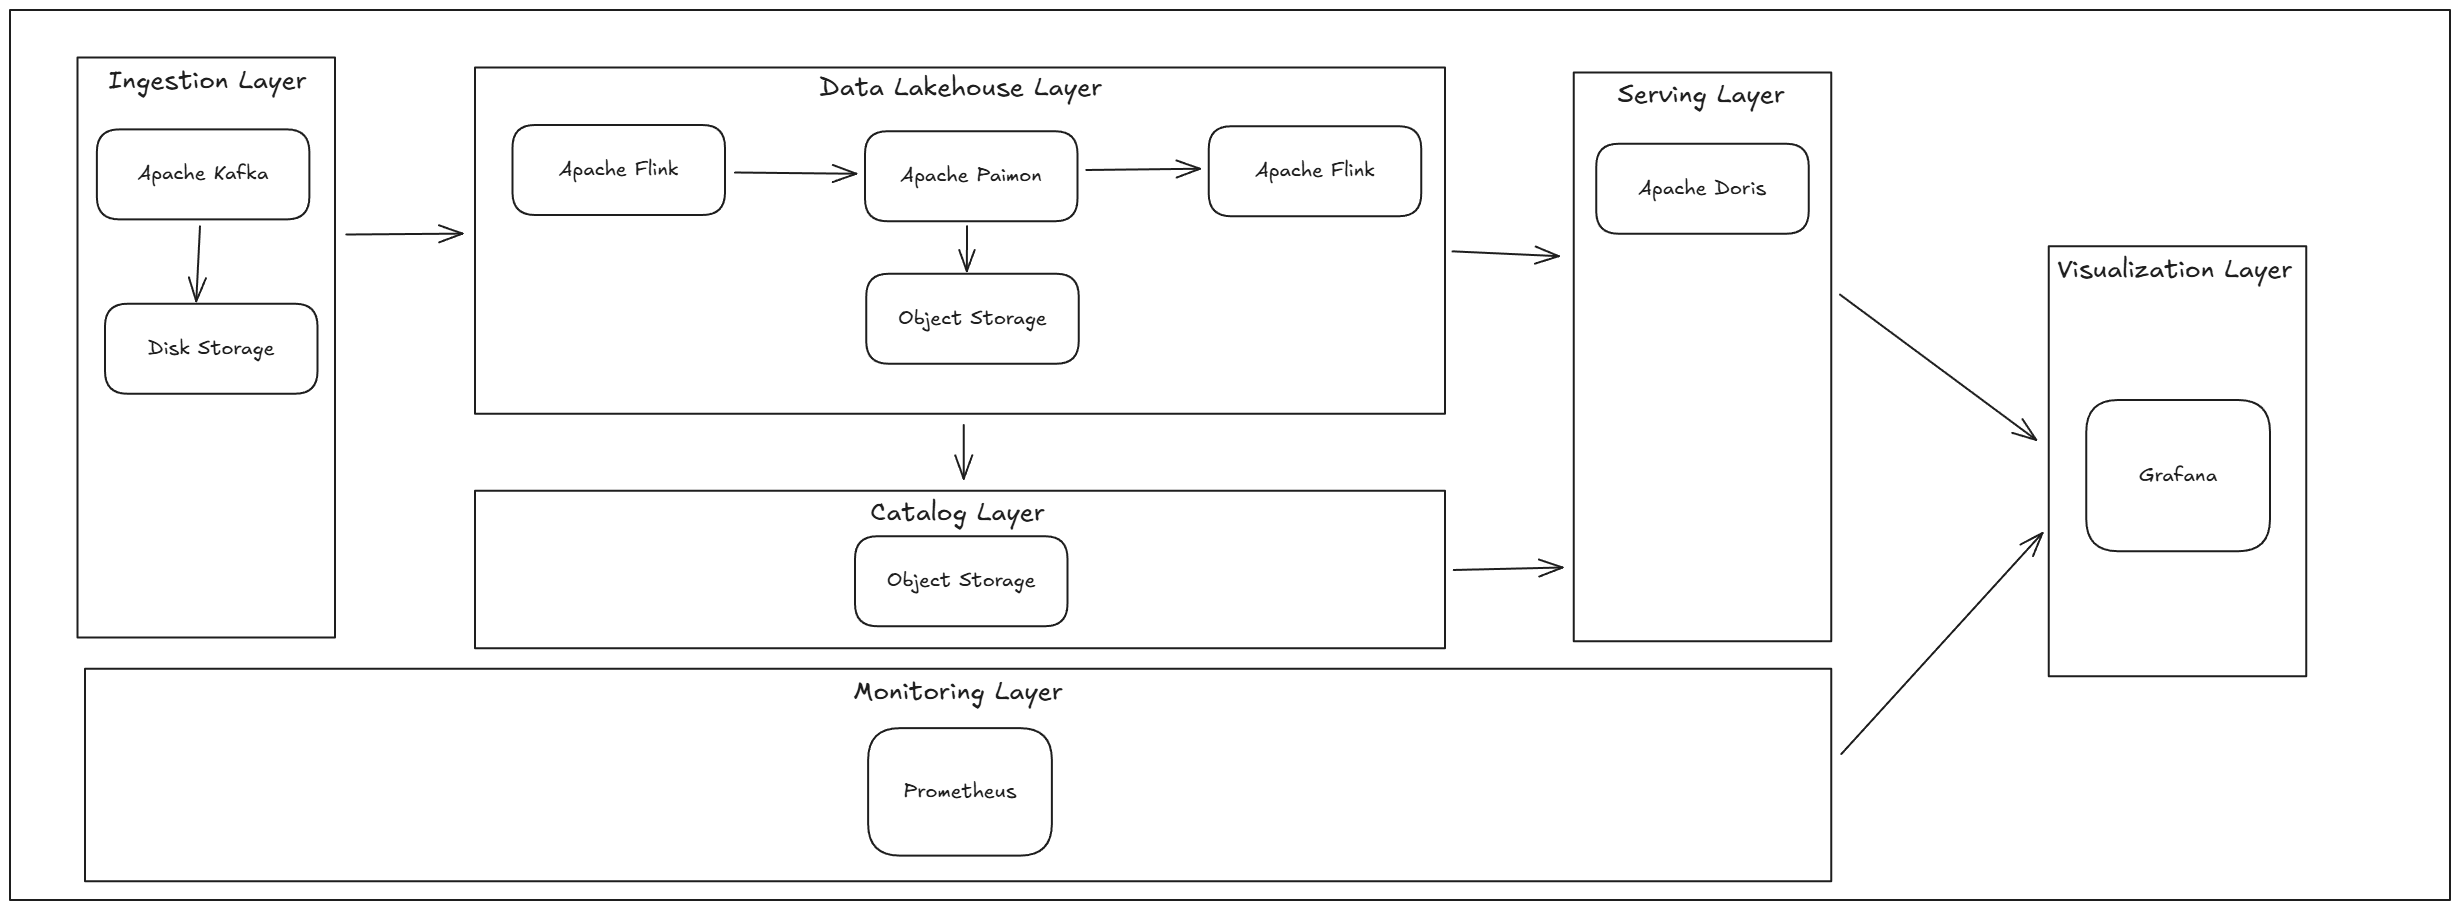
\includegraphics[width=\paperwidth]{desarrollo/Delta.png}}
    \caption{Diagrama de la Arquitectura Delta}
    \label{fig:des_arquitectura_delta}
\end{figure}

\clearpage
\newpage

\subsection{Flujo de Procesamiento}

El siguiente es un ejemplo de uno de los trabajos de procesamiento de datos desarrollados:

\begin{lstlisting}[language=sql]
    SET 'execution.runtime-mode' = 'streaming';
    SET 'execution.checkpointing.mode' = 'EXACTLY_ONCE';
    SET 'table.local-time-zone' = 'UTC';
    SET 'execution.checkpointing.interval' = '60000';
    SET 'execution.checkpointing.timeout' = '30000';
    SET 'state.backend' = 'hashmap';
    SET 'table.exec.state.ttl' = '300000';
    SET 'parallelism.default' = '2';

    CREATE CATALOG paimon WITH (
        'type' = 'paimon',
        'warehouse' = 's3://datalake/paimon',
        's3.endpoint' = 'http://minio:9000',
        's3.access-key' = 'minioadmin',  
        's3.secret-key' = 'minioadmin',
        's3.path.style.access' = 'true',
        'location-in-properties' = 'true'
    );
\end{lstlisting}

\begin{lstlisting}[language=sql]
    CREATE TABLE paimon.delta.raw_measurements (
        measurement_timestamp TIMESTAMP(3),
        measurement_type STRING,
        raw_value STRING,
        device_id STRING,
        battery DOUBLE,
        signal_strength DOUBLE,
        ingestion_timestamp TIMESTAMP(3),
        WATERMARK FOR measurement_timestamp AS measurement_timestamp - INTERVAL '10' SECONDS
    );
\end{lstlisting}

\newpage

\begin{lstlisting}[language=sql]
    CREATE TABLE default_catalog.default_database.raw_measurements (
        measurement_timestamp TIMESTAMP(3),
        measurement_type STRING,
        raw_value STRING,
        device_id STRING,
        battery DOUBLE,
        signal_strength DOUBLE,
        ingestion_timestamp TIMESTAMP(3) METADATA FROM 'timestamp' VIRTUAL,
        WATERMARK FOR measurement_timestamp AS measurement_timestamp - INTERVAL '10' SECONDS
    ) WITH (
        'topic' = 'raw.measurements',
        'connector' = 'kafka',
        'properties.bootstrap.servers' = 'kafka-1:19091,kafka-2:19092,kafka-3:19093',
        'format' = 'json',
        'json.timestamp-format.standard' = 'ISO-8601',
        'scan.startup.mode' = 'latest-offset'
    );
\end{lstlisting}

\begin{lstlisting}[language=sql]
    INSERT INTO paimon.delta.raw_measurements
    SELECT * FROM default_catalog.default_database.raw_measurements;
\end{lstlisting}

Este código muestra algunas de las características principales del uso de Flink SQL en conjunto con Paimon.
Las primeras tres reglas son las estándares para un procesamiento de streaming 
con manejo de mensajes en tiempo real y que además utilice una hora estándar para tener sincronizadas
las marcas de tiempo de todos los sistemas que intervienen.\newline

Luego se define el 'execution.checkpointing.interval' que es de los parámetros más importantes para el procesamiento de streaming,
ya que define cada cuanto tiempo se guardan los estados intermedios de los datos procesados.
Para el caso de Paimon particularmente, marca cada cuanto se impactan los datos procesados en el almacenamiento,
por lo que define que tan pronto estarán disponibles estos para su consumo.\newline

Esto afecta directamente a la latencia, por lo que es algo que se tiene que balancear fuertemente con 
los recursos del sistema para evitar retrasos en el procesamiento.\newline

\newpage

Algo importante a destacar es que si bien en este caso se define el catalogo en cada uno de los scripts, 
esto no debería ser necesario pues Flink permite definir mediante configuración sus catálogos disponibles.
Sin embargo, no fue posible configurarlo de esta manera, por lo que se optó por definirlo en cada uno de los scripts.\newline

Un último detalle a destacar, es que se define el paralelismo en 2 de modo tal que se pueda aprovechar al máximo 
las particiones del tópico de Kafka. Lo ideal sería definirlo en 3, 
pero esto no es posible por una limitante de hardware en cuanto a memoria en el nodo que ejecuta el trabajo de procesamiento.\newline

Esta primer inserción de datos que se encarga de recibir los datos en formato JSON desde el tópico de Kafka
y almacenarlos en el formato de Paimon es una de las dos grandes diferencias de esta arquitectura respecto a la anterior.
La segunda diferencia es que en este caso no es necesaria la inserción en Doris, ya que esta es sólo una herramienta que se usa para acceder a los datos pero no los almacena. 
Esto hace que el flujo de procesamiento sea más simple y liviano al no haber un tercer componente que tenga que procesar información. 